\section{System}\label{sec:System}
\todo[inline, color=yellow]{Vera}
This chapter describes the contour searching method and different approaches to detect the light direction of an object in detail. In the beginning, the contours of an object of interest are generated in the application to get all pixel coordinates along an adequate contour patch. Followed by the actual computations to ascertain the light direction of an infinitive light source that shines on the object belonging to the contour patch.

\subsection{Contours}\label{sec:contours}
\todo[inline, color=yellow]{Vera}
To estimate the light direction of an object in a digital image, it is firstly needed to locate the object of interest and get its shape informations. All informations are described by the contour which is forced to be perfectly even to guarantee a successful light direction estimation. The most important required informations are all pixel coordinates along the outer bound of the object in an ordered way. 

Beside a correctly localisation, an application with a good usability is preferred as well. An pre implemented interactive segmentation \cite{website:LiveWire} was integrated into the application to generate the affordable contours with manual constraints that are defined by the user. This method is called \textit{Live-Wire}~\cite{BARRETT1997331} and based on a maximum flow problem. However, several test showed that this extension calculates noisy and fault contours as well as lacks of a robust use control. The main problem was that the generated contour seems to follow the valley between two edges of an RGB image and snap to the most significant edge in a wide neighbourhood. Even more constraints set by the user did not result in adequate and useful shapes. 

According to this bad results, the team decided to extract the contours from perfectly even mask images of the objects of interest like in in Figure \ref{fig:batch1mask}. These images are made manually in \textit{Adobe Photoshop CS 6} with the pen tool that offers perfectly round and even Bezier curves. All created masks are shrink about almost two pixels to ensure that only pixel informations of the actual object are used for further proceedings and none from the background. 

If the file name of a mask image is the same as the one belonging to the selected RGB image with the extension \texttt{\_mask.jpg}, it will be loaded automatically into the application at the same time when the belonging RGB image is opened. This mask data will be used for all further contour calculations.

\begin{figure} [H]
	\center 
	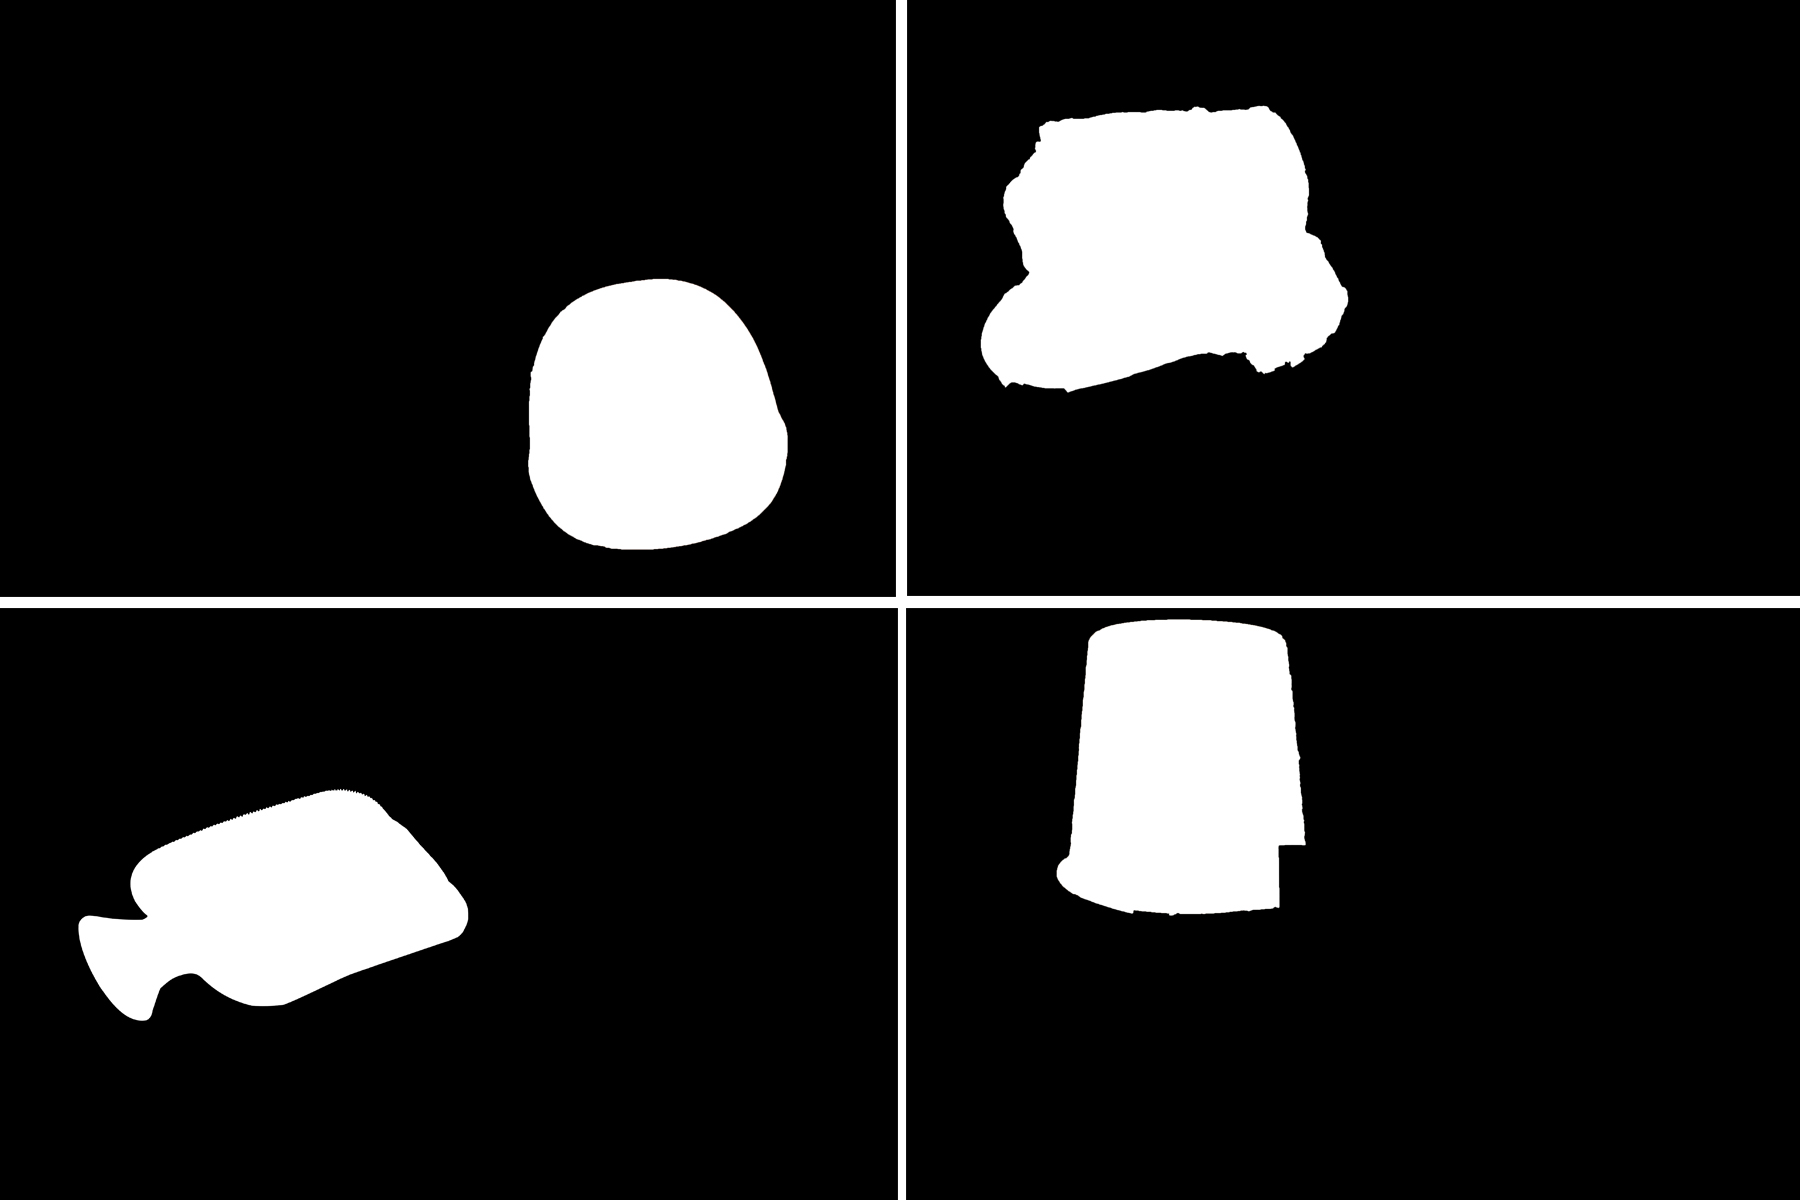
\includegraphics[width=12cm]{Images/batch1_mask.jpg}			
	\caption[Bildunterschrift]{Manual created mask images of the first batch.}
	\label{fig:batch1mask}
\end{figure}

\subsubsection{Calculate Contours}\label{sec:findContours}
\todo[inline, color=yellow]{Vera}

Several \textit{OpenCV} functions are used to compute all required pixel coordinates along the outer object bound. In the beginning a common erosion filter with a filter size of three is applied to the mask image to eliminate small outliers and to shrink the mask to ensure that it is not located directly or outside the object bound. In the next step, a Canny filter with a filter size of five is used to extract the edges. Then the \textit{OpenCV} function \texttt{findContours()} calculates the vector representations of the binary canny image with the border following algorithm of Suzuki et Al.~\cite{SUZUKI198532}. All results are not optimized by any approximations because otherwise important coordinate data will be lost. The resulting contours will be printed into the preview of the GUI to allow the user a selection of a suitable sub-contour to feed the light direction estimation.

\subsection{Generate Subcontours}\label{sec:subcontours}
\todo[inline, color=yellow]{Vera}

As mentioned, the user is forced to select an adequate part of the contour to contain the further calculations. He can do so in the GUI with a simple rectangle selection in the preview. This selection can be renewed, if affordable, and saved. After the storage of all contour points within the rectangle, they are stored and sorted in a so called  sub-contour. At this point, the sort is needed because all contour points are stored like a ring buffer that starts at the highest point and then follows counter clock wise the boundary. Thus, it has to be reordered to ensure an open and gapless sub-contour, if the selection includes the top of the complete contour.

After this process, we have an sub-contour that includes all important edge points along the boundary but it still lacks of all pixel coordinates along this part of the boundary.
This circumstance can be solved by making a binary image and print the required sub-contour into it with a line thickness of one pixel. Then a \textit{OpenCV} \texttt{LineIterator} is applied to this image. It is treated as versatile implementation of the Bresenham algorithm~\cite{5388473} and allows the notice and storage of every required coordinate. Now, these coordinates can be used for the following approaches of the light direction estimation in a single digital image.


\subsection{Illumination Model}\label{sec:lightingmodel}
\todo[inline, color=yellow]{Vera}
To understand the following approaches, it is useful to give a short introduction to the definition of an illumination model. One of the most acknowledged illumination model is the Blinn model~\cite{Blinn:1977}(see Equation \ref{equ:Blinn}) which defines a basic illumination in a three dimensional space. This illumination is a sum of ambient $a$, diffuse $d$ and specular $sp$ light parts where $\vec{n}$ is the surface normal, $\vec{l}$ is the light direction vector and $\vec{h}$ is the direction of the maximum highlights. The $p$ are variables that are related to the proportions of each reflection type which are part of the sum and $s$ is the amount of the specular reflection.

\begin{equation}
\label{equ:Blinn}
I(x,y,z) = (\vec{n}\cdot \vec{l})*p_d + (\vec{n}\cdot\vec{h})^s*p_s + p_a = d + sp + a
\end{equation} 

Due to the high number of unknown variables and vectors, the Blinn model is too complex to calculate the 3-vector $\vec{l}$ with standard approaches like the least square method. Hence, some assumptions to simplify the mode had to be made~\cite{Johnson}. The first assumption is to state the current surface reflects light isotropically. This surface has a constant reflectance value $r$ and is illuminated by a faraway infinitive light source. Finally, the angle between $\vec{n}$ and  $\vec{l}$ is in the range of $0^\circ $ and $90^\circ$. All previous assumptions lead to the simplified light model of equation \ref{equ:simpleLightmodel}.

\begin{equation}
\label{equ:simpleLightmodel}
I(x,y,z) = r(\vec{n}\cdot \vec{l}) + a
\end{equation} 

\subsection{Different Approaches}\label{sec:approaches}
\todo[inline, color=yellow]{Laura}
Because no reliable solution could be found, three different approaches were tried out. 
All three approaches are based on the paper of Johnson and Farid \cite{Johnson}. 
Whereas two of this approaches remained unchanged (compare section~\ref{sec:appOne} and \ref{sec:appTwo}), the last approach takes the assumptions of Johnson and Farid and expand them (compare section~\ref{sec:appThree}). \\
To standardise the explanations in the following sections a list of necessary variables is introduced: 
\begin{itemize}
\item $\vec{L}$: vector, which points in the direction of the light source (3D)
\item $\vec{N}(x,y)$: surface normal at the point (x,y) (3D)
\item $I(x,y)$: intensity at the point (x,y)
\item $A$: constant ambient light term
\item $R$: constant reflectance value
\end{itemize}
All equations in this section, as well as its subsections, are taken from \cite{Johnson}. The basic idea behind the approach of Johnson and Farid is summed up in equation \ref{equ:General}.

\begin{equation}
\label{equ:General}
I(x,y) = R(\vec{N}(x,y)\cdot \vec{L}) + A
\end{equation}

In the following sections we do not have a three dimensional room, as all evaluations are made based on images. All of them have in common, that their assumptions are based on a infinite light source in a two dimensional image space. Therefore $\vec{L}$ and $\vec{N}(x,y)$ needs to be redefined as follows:
\begin{itemize}
\item $\vec{L}$: vector, which points in the direction of the light source (2D)
\item $\vec{N}(x,y)$: surface normal at the point (x,y) (2D)
\end{itemize}

For the second and the third approach, the light vectors are summed up in patches of size four. 

\subsubsection{1. Approach: One Lightvector}\label{sec:appOne}
\todo[inline, color=yellow]{Laura}
The first approach tries to simplify the two dimensional case by solving equation \ref{equ:firstApp} and getting one final light vector per contour of an object plus the ambient light term. The Matrix $M$ can be found in Johnsons and Farids paper \cite{Johnson} in equation (6) and $p$ denotes the number of points on a contour with the same assumed reflectance. All other variables are explained in section~\ref{sec:approaches}. Thereby the reflectance along the entire contour is thought of as constant. 

\begin{equation}
\label{equ:firstApp}
E(\vec{L} , A) = 
\left\vert \left\vert 
M
\begin{pmatrix}
L_{x} \\
L_{y} \\
A \\
\end{pmatrix} -
\begin{pmatrix}
I(x_{1} , y_{1}) \\
I(x_{2} , y_{2}) \\
\vdots \\
I(x_{p} , y_{p}) \\
\end{pmatrix}
 \right\vert\right\vert^{2}
 = \left\vert \left\vert  M\vec{v}-\vec{b}  \right\vert\right\vert^{2}
\end{equation}

This options can be activated in our script \textit{mainwindow.cpp} by setting \textit{usePatches} to \textit{false}. Equation~\ref{equ:firstApp} is than solved using \textit{Singular Value Decomposition}. Then the lightvector $\vec{L}$ is drawn onto the test image to visualize the result.  

\subsubsection{2. Approach: Averaging Lightvectors}\label{sec:appTwo}
\todo[inline, color=yellow]{Laura}
For the second approach it is not only assumed, that the light source is infinite, but also that the reflection created by it is constant within each surface patch. The basic idea can be found in section 2.2.1 in the paper of Johnson and Farid \cite{Johnson}.\\
It is assumed, that a minimization problem according to equation~\ref{equ:secondApp} needs to be solved. The Matrix $M$ can be found in \cite{Johnson} in equation (8). \\

\begin{equation}
\label{equ:secondApp}
E_{1}(\vec{L}^{\,1} , ... , \vec{L}^{\,n} , A) = 
\left\vert \left\vert 
M
\begin{pmatrix}
L^{1}_{x} \\
L^{1}_{y} \\
\vdots  \\
L^{n}_{x} \\
L^{n}_{y} \\
A \\
\end{pmatrix} -
\begin{pmatrix}
I(x^{1}_{1} , y^{1}_{1}) \\
\vdots  \\
I(x^{1}_{p} , y^{1}_{p}) \\
\vdots  \\
I(x^{n}_{1} , y^{n}_{1}) \\
\vdots  \\
I(x^{n}_{p} , y^{n}_{p}) \\
\end{pmatrix}
 \right\vert\right\vert^{2}
 = \left\vert \left\vert  M\vec{v}-\vec{b}  \right\vert\right\vert^{2}
\end{equation}
This options can be activated in our script \textit{mainwindow.cpp} by setting \textit{usePatches} to \textit{true} and \textit{useHighestIntensity} to \textit{false}.
As stated in section~\ref{sec:appOne} equation~\ref{equ:secondApp} is solved using \textit{Singular Value Decomposition} as well. This leads to calculating one light vector per patch. To get the final vector $\vec{L}$ all of this light vectors are averaged.


\subsubsection{3. Approach: Lightvector with highest Intensity}\label{sec:appThree}
\todo[inline, color=yellow]{Laura}
This last approach uses the same basic idea as the second one described in section \ref{equ:secondApp}. It is also based on dividing the surface normals $\vec{N}$ into patches and solving equation~\ref{equ:secondApp} using \textit{Singular Value Decomposition}. Afterwards there is no averaging done, but the vector $\vec{L}$ belonging to the patch with the highest intensities is taken as the final light vector. \\
This idea is not described in the paper of Johnson and Farid~\cite{Johnson}. It was a try to make the results of the \textit{Interactive Lighting Detector} more trustworthy. \\
This options can be activated in our script \textit{mainwindow.cpp} by setting \textit{usePatches} to \textit{true} and \textit{useHighestIntensity} to \textit{true}.

\newpage